% =============================================================================
% Chuong 4: De xuat — CTAV va tac tu RCA
% =============================================================================
% Cach dung tren Overleaf:
%   1. Bao dam da tai macros.tex, refs.bib, chapters/ch4.tex va 5 anh trong
%      figures/ch4/ (h4.1-architecture.png, h4.4-ctav-design-vs-final.png,
%      h4.5-c1-2hop-fusion.png, h4.6-decision-policy.png, h4.10-rca-agent.png).
%   2. Trong main.tex:
%        \input{macros}
%        ...
%        \include{chapters/ch4}
%        ...
%        \bibliographystyle{IEEEtran}
%        \bibliography{refs}
%
% Cac nhan lien chuong duoc tham chieu tu Chuong 4:
%   Chuong: ch:mo-dau, ch:nen-tang, ch:cong-trinh-lien-quan, ch:thuc-nghiem,
%           ch:platform, ch:thao-luan
%   Chuong 2: sec:ch2-du-lieu, sec:ch2-phat-hien, sec:ch2-truy-xuat,
%             sec:ch2-judge, sec:ch2-rca, sec:ch2-dang-ky, sec:ch2-cong-nghe
%   Chuong 3: sec:ch3-khoang-trong
%   Chuong 5: sec:ch5-hypotheses, sec:ch5-data, sec:ch5-setup, sec:ch5-gport,
%             sec:ch5-gpaper, sec:ch5-val, sec:ch5-h1, sec:ch5-c5, sec:ch5-test,
%             sec:ch5-ablation, sec:ch5-budget, sec:ch5-rca
%   Chuong 7: sec:ch7-errors
% =============================================================================

\section{Đề xuất: \CTAV{} và tác tử \term{RCA}{RCA}}
\label{ch:de-xuat}

Chương này trình bày thiết kế chi tiết của phương pháp thẩm định cảnh báo hiệu chỉnh có nhận biết topology (\CTAV{} — \emph{Calibrated Topology-Aware Alert Validation}), tác tử phân tích nguyên nhân gốc (\term{RCA}{RCA}) và kiến trúc nền tảng hiện thực hóa hai thành phần này nhằm giải quyết bốn khoảng trống nghiên cứu từ Mục~\ref{sec:ch3-khoang-trong}. Mục~\ref{sec:ch4-mo-ta} mô tả kiến trúc tổng thể bốn khâu, phát biểu hình thức bài toán và phân tích năm thách thức thiết kế chính. Mục~\ref{sec:ch4-detector} trình bày bộ phát hiện bất thường Isolation Forest cùng cổng cứu cảnh báo \textbf{\comp{C5}} (\code{Rescue Score}, chỉ đánh giá ở vai trò ablation). Mục~\ref{sec:ch4-ctav} đi sâu vào không gian thiết kế của \CTAV{}, phân biệt rành mạch hai thành phần lõi giữ lại trong cấu hình cuối là truy xuất lai \term{BM25}{BM25}--topology (\textbf{\comp{C1}}) và neo bằng chứng bất thường (\textbf{\comp{C3}}) với hai thành phần đã kiểm chứng rồi loại trên tập \splitname{val} là ngưỡng bất đối xứng theo nguồn bằng chứng (\textbf{\comp{C2}}) và định tuyến hai tầng thích nghi (\textbf{\comp{C4}}). Mục~\ref{sec:ch4-rca} mô tả ba bước khép kín của tác tử \term{RCA}{RCA} từ gom nhóm cảnh báo, lan truyền ngược 1 bước theo chiều gọi đến sinh báo cáo JSON có kiểm duyệt. Mục~\ref{sec:ch4-impl} trình bày cách lắp ráp mã nguồn, kho lưu trữ, API và harness thực nghiệm tái lập; cuối cùng, Mục~\ref{sec:ch4-ket-chuong} tổng kết cấu hình chốt trước khi chuyển sang kiểm định ở Chương~\ref{ch:thuc-nghiem}.

% -----------------------------------------------------------------------------
\subsection{Mô tả đề xuất}
\label{sec:ch4-mo-ta}

Mục này xác lập khung tổng thể của hệ thống đề xuất, định nghĩa hình thức đầu vào--đầu ra cùng các ký hiệu toán học dùng xuyên suốt chương, và đối chiếu trực tiếp năm thách thức kỹ thuật với các thành phần giải quyết tương ứng.

\subsubsection{Tổng quan về đề xuất}
\label{sec:ch4-tong-quan}

Đề tài thiết kế một nền tảng AIOps khép kín gồm bốn khâu nối tiếp nhau: (1) phát hiện bất thường chuỗi thời gian trên metric, (2) thẩm định cảnh báo bằng \CTAV{} dựa trên bằng chứng đa phương thức (metric, log, trace), (3) tác tử phân tích nguyên nhân gốc trên các cảnh báo đã xác nhận, và (4) tầng lưu trữ, API cùng bảng điều khiển phục vụ trực quan hóa. Như minh họa ở Hình~\ref{fig:ch4-arch}, toàn bộ luồng thực nghiệm và luồng trình diễn đều chạy trên cùng một pipeline thống nhất; trong đó, đường xử lý chính đi từ phát lại cửa sổ telemetry 60~s qua bộ phát hiện đến \CTAV{} và tác tử \term{RCA}{RCA}, còn việc ghi bảng phân tích vào ClickHouse, bảng sự cố vào PostgreSQL và hiển thị trên dashboard được tách sang nhánh phi đường găng để không cản trở phép đo độ trễ của khâu suy luận.

\begin{figure}[htbp]
  \centering
  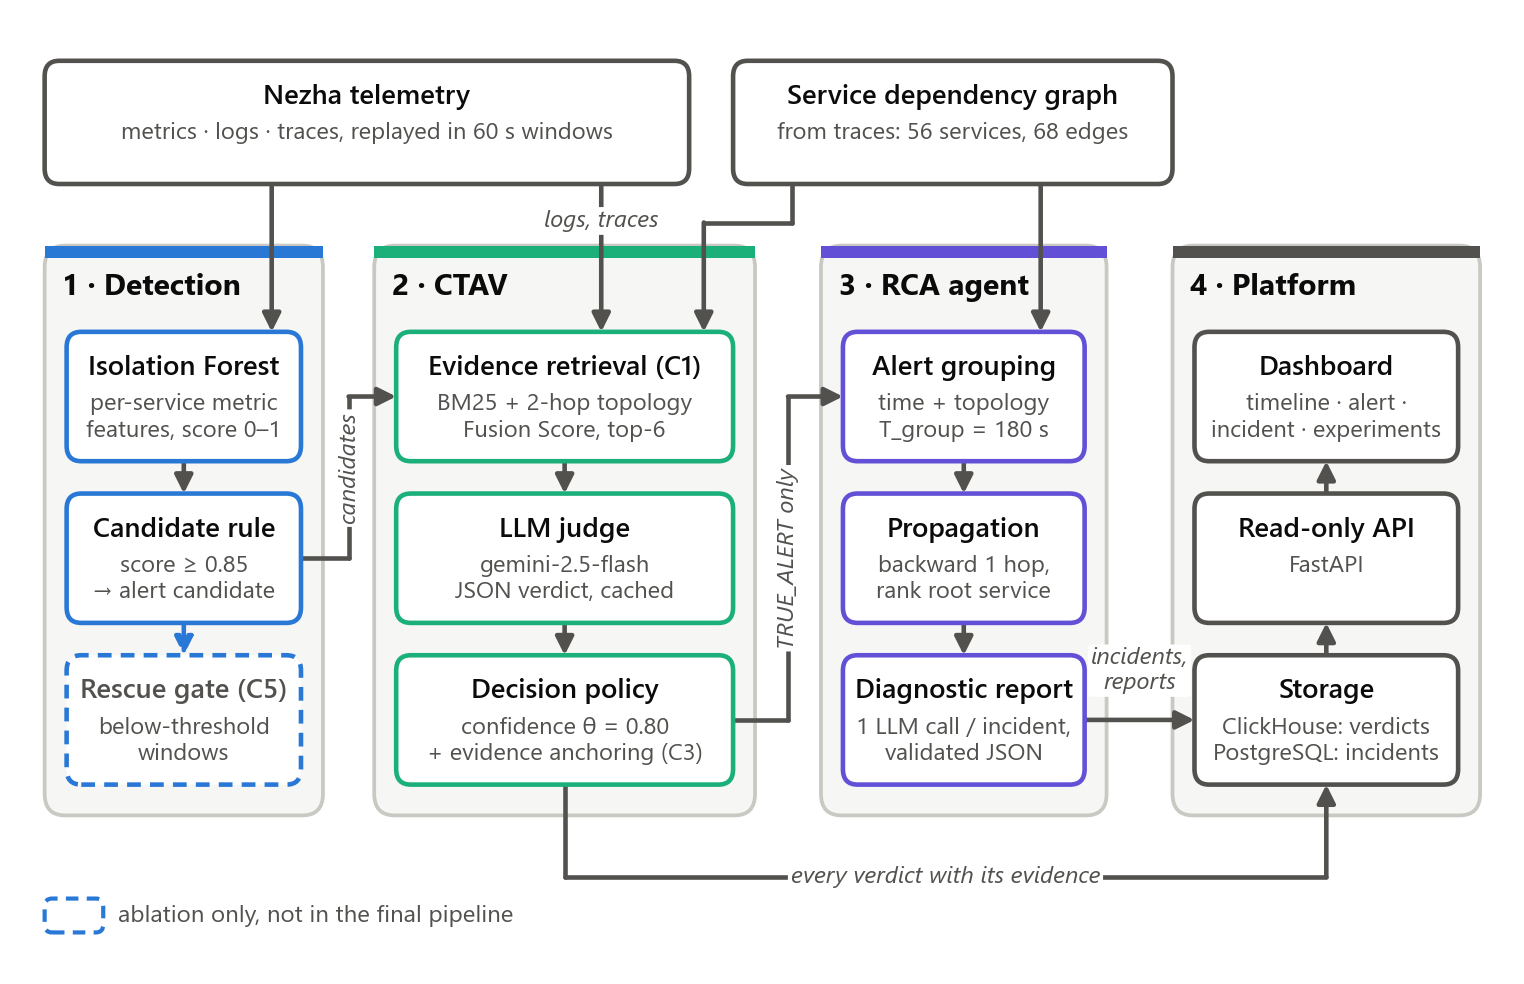
\includegraphics[width=\linewidth]{Images/C1/figures/ch4/h4.1-architecture.png}
  \vspace{0.35cm}
  \caption[Kiến trúc tổng thể bốn khâu của nền tảng ở cấu hình chốt]{Kiến trúc tổng thể bốn khâu ở cấu hình chốt: phát hiện bất thường, \CTAV{}, tác tử \term{RCA}{RCA} và platform (khối nét đứt \comp{C5} chỉ dùng cho ablation). \emph{(Nguồn: tác giả vẽ, có hỗ trợ AI.)}}
  \label{fig:ch4-arch}
\end{figure}

Để bảo đảm khả năng thay thế và kiểm định từng thành phần mà không phá vỡ luồng xử lý, kiến trúc định nghĩa bốn giao diện lõi (\code{Protocol}) cố định ở tầng lược đồ dùng chung, tóm tắt ở Bảng~\ref{tab:ch4-protocols}. Mọi tham số đặc thù của thuật toán (như số bước nhảy đồ thị, hệ số suy giảm thời gian hay ngưỡng tin cậy) đều được nạp qua hàm khởi tạo từ tệp cấu hình YAML thay vì đưa vào chữ ký phương thức. Đối với mô hình ngôn ngữ lớn đóng vai trò bộ thẩm định, kiến trúc chọn một mô hình API cố định duy nhất là \code{gemini-2.5-flash} ở nhiệt độ $0$, đi qua lớp cache bắt buộc và không dùng mô hình cục bộ dự phòng, nhằm loại bỏ sai lệch do đổi mô hình giữa các lượt chạy thực nghiệm và bảo đảm chế độ trình diễn ngoại tuyến hoàn toàn từ cache.

\begin{table}[H]
  \centering
  \caption{Bốn giao diện (\code{Protocol}) lõi và ánh xạ sang các mô-đun hiện thực.}
  \label{tab:ch4-protocols}
  \tblfont
  \tblsetup
  \setlength{\tabcolsep}{4pt}
  \begin{tabularx}{\linewidth}{|l|>{\raggedright\arraybackslash}p{3.0cm}|Y|>{\raggedright\arraybackslash}p{3.7cm}|}
    \hline
    \rowcolor{gray!15}
    \textbf{Protocol} & \textbf{Phương thức chính} & \textbf{Đầu vào / Đầu ra} & \textbf{Thành phần hiện thực} \\
    \hline
    \code{SourceAdapter} & \code{stream()} & Nguồn dữ liệu $\to$ luồng \code{TelemetryWindow} 60~s theo watermark & Bộ phát lại dữ liệu Nezha \\
    \hline
    \code{Detector} & \code{score()}, \code{is\_candidate()} & \code{TelemetryWindow} $\to$ điểm bất thường $[0, 1]$ và cờ ứng viên & Bộ phát hiện Isolation Forest \\
    \hline
    \code{RetrievalStrategy} & \code{retrieve(\allowbreak candidate, budget)} & \code{AlertCandidate}, \code{RetrievalBudget} $\to$ \code{RetrievalResult} & Truy xuất \term{BM25}{BM25} cục bộ, \comp{C1} lai đồ thị và đối chứng không ngữ cảnh \\
    \hline
    \code{Judge} & \code{evaluate(\allowbreak candidate, context)} & \code{AlertCandidate}, \code{RetrievalResult} $\to$ \code{JudgedAlert} & Bộ thẩm định LLM qua cache bất biến \\
    \hline
  \end{tabularx}
\end{table}

\subsubsection{Các vấn đề nghiên cứu}
\label{sec:ch4-van-de}

Xét một hệ microservice được biểu diễn bởi đồ thị phụ thuộc có hướng $G = (V, E)$, trong đó tập đỉnh $V$ là các service và cạnh có hướng $(u, v) \in E$ biểu thị service $u$ gọi service $v$ quan sát được từ cặp \code{SpanID}--\code{ParentID} trong trace. Dữ liệu quan sát đa phương thức được cắt thành các cửa sổ không chồng lấn $w$ có độ dài $60\,\text{s}$, mỗi cửa sổ gắn với một service $s_0 \in V$, pod tương ứng và mốc trung điểm $t_0$. Nhãn thực tế $y(w) \in \{\text{fault}, \text{normal}\}$ được gán theo thời gian thực (\emph{wall-clock}) quanh thời điểm tiêm lỗi như định nghĩa ở Mục~\ref{sec:ch2-du-lieu}.

\textbf{Bài toán nhánh A (Thẩm định cảnh báo dưới ngân sách LLM).} Từ luồng cửa sổ telemetry, bộ phát hiện sinh tập cảnh báo ứng viên $c = (w, s_0, t_0, \text{score}_{\text{det}}, \text{source})$ với $\text{source} \in \{\text{metric}, \text{rescue}\}$. Với mỗi ứng viên $c$, chiến lược truy xuất chọn tập bằng chứng $E(w)$ gồm tối đa $k$ sự kiện log/trace trong ngân sách token định trước, rồi bộ thẩm định kết hợp chính sách quyết định ánh xạ $(w, E(w))$ sang nhãn phán quyết cuối:
\begin{equation}
  \hat{y}(w) \in \{\code{TRUE\_ALERT},\; \code{FALSE\_POSITIVE},\; \code{UNCERTAIN}\},
  \label{eq:ch4-verdict-space}
\end{equation}
kèm điểm tin cậy $p(w) \in [0, 1]$ và tập định danh bằng chứng trích dẫn $C(w) \subseteq E(w)$. Dưới ràng buộc tổng số lần gọi LLM không vượt quá ngân sách $B$, mục tiêu tối ưu của \CTAV{} là giữ được mức tăng thu hồi (Recall) nhờ ngữ cảnh topology của \comp{C1} so với truy xuất cục bộ \term{BM25}{BM25} mà không làm tăng tỷ lệ báo động giả (\term{FPR}{FPR}), tức đồng thời thỏa:
\begin{equation}
  \Delta\text{F1}(\text{\CTAV} - \text{BM25}) > 0, \;
  \Delta\text{FPR}(\text{\CTAV} - \text{BM25}) \le 0, \;
  \Delta\text{Recall}(\text{\CTAV} - \text{C1}) \ge -\delta,
  \label{eq:ch4-ctav-objective}
\end{equation}
với biên chấp nhận giảm thu hồi $\delta = 0{,}05$ đã đăng ký trước cho giả thuyết chính \hyp{H2} (Mục~\ref{sec:ch5-hypotheses}).

\textbf{Bài toán nhánh B (Phân tích nguyên nhân gốc).} Cho tập các cảnh báo đã được \CTAV{} xác nhận $A_{\text{conf}} = \{c \mid \hat{y}(w_c) = \code{TRUE\_ALERT}\}$ và đồ thị phụ thuộc $G$, tác tử \term{RCA}{RCA} cần thực hiện hai ánh xạ nối tiếp: (i) phân hoạch $A_{\text{conf}}$ thành các sự cố $I_1, I_2, \dots, I_m$ theo độ gần thời gian và tính liên thông topology để giảm tải cảnh báo (đo bằng \emph{Alert Reduction Ratio}, \term{ARR}{ARR}); và (ii) với mỗi sự cố $I$, xếp hạng danh sách service nghi vấn gốc $\hat{r}(I) = (v_1, v_2, \dots)$ (đo bằng $\text{Hit}@1$, $\text{Hit}@3$) rồi sinh báo cáo chẩn đoán JSON hợp lệ kèm bằng chứng trích dẫn. Hai bài toán này gắn trực tiếp với năm câu hỏi nghiên cứu ở Chương~\ref{ch:mo-dau}: \rqref{RQ1} kiểm chứng hiện tượng đánh đổi của truy xuất topology và cơ chế \term{ConfirmationBias}{thiên lệch xác nhận}; \rqref{RQ2} và \rqref{RQ3} đánh giá hiệu quả tổng thể và đóng góp riêng lẻ của từng thành phần \comp{C1}--\comp{C5} trong \CTAV{}; \rqref{RQ4} khảo sát độ bền của \CTAV{} theo ngân sách lời gọi $B$; và \rqref{RQ5} đánh giá khả năng định vị gốc cùng chất lượng báo cáo của tác tử \term{RCA}{RCA}. Các ký hiệu chính dùng trong toàn bộ Chương~\ref{ch:de-xuat} được hệ thống hóa trong Bảng~\ref{tab:ch4-ky-hieu}.

\begin{table}[H]
  \centering
  \caption{Bảng ký hiệu toán học dùng trong phát biểu bài toán và thiết kế thuật toán.}
  \label{tab:ch4-ky-hieu}
  \tblfont
  \tblsetup
  \begin{tabularx}{\linewidth}{|l|Y|l|}
    \hline
    \rowcolor{gray!15}
    \textbf{Ký hiệu} & \textbf{Ý nghĩa} & \textbf{Giá trị / Miền} \\
    \hline
    $w,\; s_0,\; t_0$ & Cửa sổ telemetry 60~s, service phát cảnh báo và mốc trung điểm của cửa sổ & $s_0 \in V$ \\
    \hline
    $G = (V, E),\; d_G(u, v)$ & Đồ thị phụ thuộc service từ trace và khoảng cách bước nhảy vô hướng & $56$ nút, $68$ cạnh \\
    \hline
    $E(w),\; C(w)$ & Tập bằng chứng truy xuất (tối đa $k = 6$) và tập bằng chứng judge trích dẫn & $C(w) \subseteq E(w)$ \\
    \hline
    $\alpha, \beta, \gamma,\; \tau_F$ & Trọng số và hằng số suy giảm thời gian của \term{FusionScore}{Fusion Score} (\comp{C1}) & $0{,}35;\; 0{,}25;\; 0{,}40;\; 300\,\text{s}$ \\
    \hline
    $\theta_{\text{local}},\; \theta_{\text{topo}}$ & Ngưỡng tin cậy của chính sách quyết định (\comp{C2} dùng $\theta_{\text{topo}}$, đã loại) & $0{,}80$ ($0{,}85$ cho \comp{C2}) \\
    \hline
    $\eta_1, \eta_2, \eta_3,\; \tau$ & Trọng số ba thành phần và ngưỡng kích hoạt của \term{RescueScore}{Rescue Score} (\comp{C5}) & $(0;\, 0{,}4;\, 0{,}6)$;\; $\tau = 0{,}8$ \\
    \hline
    $T_{\text{group}}$ & Cửa sổ cắt cụm thời gian liên kết đơn khi gom cảnh báo thành sự cố & $180\,\text{s}$ \\
    \hline
    $B$ & Ngân sách tối đa số lần gọi API LLM trong một lượt chạy thẩm định & $\{120, \dots, \text{đủ}\}$ \\
    \hline
  \end{tabularx}
\end{table}

\subsubsection{Các thách thức và khó khăn}
\label{sec:ch4-thach-thuc}

Hiện thực hóa mục tiêu~\eqref{eq:ch4-ctav-objective} cùng nhánh \term{RCA}{RCA} trên dữ liệu quan sát thực tế đối mặt với năm thách thức thiết kế chính:
\begin{enumerate}
  \item \textbf{T1 — Cân bằng \term{FPR}{FPR} và Recall:} Chính sách chặn báo động giả quá chặt dễ hạ nhầm các lỗi thiếu log tường minh (như trễ mạng); \CTAV{} kiểm soát đánh đổi này bằng cặp \comp{C1} + \comp{C3} và ghi nhận minh bạch mức giảm recall ở Chương~\ref{ch:thuc-nghiem}.
  \item \textbf{T2 — Cơ chế thiên lệch khác giả thuyết trực giác:} Phân tích \hyp{H1} trên \splitname{val} (Mục~\ref{sec:ch5-h1}) cho thấy báo động giả không đến từ nhiễu lân cận như giả định tiền đề~\cite{icaetm2026}, mà từ \term{ConfirmationBias}{thiên lệch xác nhận}~\cite{sharma2024sycophancy} trên trace span cục bộ sát $t_0$, buộc thiết kế chuyển từ lọc khoảng cách đồ thị (\comp{C2}) sang kiểm tra tính bất thường định lượng tại chính $s_0$ (\comp{C3}).
  \item \textbf{T3 — Giới hạn ngân sách và tái lập:} Hệ thống dùng cache bất biến khóa \code{sha256} và tách chính sách quyết định thành hàm thuần trên phán quyết đã lưu cache để chạy ablation với $0$ lượt gọi mới.
  \item \textbf{T4 — Cảnh báo đầu vào thưa ở tầng \term{RCA}{RCA}:} Sau khi \CTAV{} lọc mạnh FP, chuỗi cảnh báo sang \term{RCA}{RCA} thường thưa; tác tử \term{RCA}{RCA} tách tầng thuật toán tất định khỏi tầng tóm tắt LLM có kiểm duyệt để dễ cô lập nguyên nhân sai (Mục~\ref{sec:ch5-rca}).
  \item \textbf{T5 — Kỷ luật chống rò rỉ:} Chia split theo \code{injection\_id} kèm vùng đệm $600\,\text{s}$, đăng ký trước \hyp{H0}--\hyp{H5} và đóng băng cấu hình trước khi chạy \splitname{test} đúng một lần.
\end{enumerate}

% -----------------------------------------------------------------------------
\subsection{Isolation Forest và cổng Rescue (\comp{C5})}
\label{sec:ch4-detector}

Mục này trình bày tầng đầu tiên của pipeline: bộ phát hiện bất thường chuỗi thời gian Isolation Forest tạo tập ứng viên cho \CTAV{}, cùng cơ chế cổng cứu cảnh báo \comp{C5} (\code{Rescue Score}) dùng để kiểm chứng khả năng thu hồi các cửa sổ bị bộ phát hiện metric bỏ sót.

\textbf{Vấn đề giải quyết.} Trên tập dữ liệu Nezha~\cite{nezha} gồm hàng chục nghìn cửa sổ 60~s với tỷ lệ mất cân bằng xấp xỉ $1:135$ giữa cửa sổ lỗi và cửa sổ bình thường, gọi trực tiếp LLM trên mọi cửa sổ là bất khả thi về chi phí lẫn độ trễ. Tầng phát hiện cần một mô hình không giám sát chạy nhanh, chỉ huấn luyện trên tập \splitname{dev} để loại bỏ phần lớn cửa sổ bình thường mà vẫn đưa đủ cửa sổ bất thường vào hàng đợi thẩm định. Ngược lại, một số dạng lỗi ứng dụng (như ngoại lệ phần mềm hoặc lỗi trả về sớm) ít gây biến động mạnh trên metric hạ tầng, đặt ra câu hỏi liệu có thể cứu lại những cửa sổ dưới ngưỡng metric bằng dấu hiệu log và đồ thị phụ thuộc hay không.

\textbf{Thiết kế bộ phát hiện Isolation Forest.} Bộ phát hiện \code{IsolationForestDetector} duy trì một bộ đệm cuộn (\emph{rolling buffer}) kích thước \code{buffer\_size = 2} riêng cho từng khóa pod (dự phòng theo tên service nếu thiếu pod), tương ứng khoảng $120\,\text{s}$ lịch sử gần nhất. Trên mỗi cửa sổ, với từng metric trong tập đặc trưng của tập huấn luyện, mô-đun trích xuất bảy thống kê: trung bình (\code{mean}), độ lệch chuẩn (\code{std}), giá trị nhỏ nhất (\code{min}), lớn nhất (\code{max}), giá trị cuối (\code{last}), độ chênh (\code{delta}) và tỷ lệ thiếu mẫu (\code{missing\_fraction}). Các metric vắng mặt trong một cửa sổ (ví dụ phân vị độ trễ \code{NaN} khi không có request) được điền bằng giá trị quan sát gần nhất của chính pod đó hoặc trung vị trên tập \splitname{dev} — tuyệt đối không điền $0{,}0$ để tránh biểu diễn nhầm một cửa sổ nhàn rỗi thành độ trễ cực thấp. Điểm bất thường từ Isolation Forest~\cite{isof} được chuẩn hóa theo phân vị trên tập huấn luyện về đoạn $[0, 1]$. Một cửa sổ chỉ trở thành ứng viên \code{AlertCandidate(source="metric")} khi bộ đệm của pod đã đầy (tránh báo động giả lúc khởi động lạnh) và thỏa:
\begin{equation}
  \text{score}_{\text{IF}}(w) \ge 0{,}85.
  \label{eq:ch4-if-rule}
\end{equation}
Ngoài điểm số, bộ phát hiện xuất ba đặc trưng có độ lệch chuẩn lớn nhất so với phân bố huấn luyện (\code{top\_features}) để đưa vào ngữ cảnh của bộ thẩm định LLM.

\textbf{\xtarget{def:C5}Thiết kế cổng cứu cảnh báo \comp{C5} (\code{Rescue Score}).} Với các cửa sổ không vượt ngưỡng~\eqref{eq:ch4-if-rule} ($y_{\text{IF}}(w) = 0$), bộ tính điểm cứu cảnh báo tính tổng trọng số dựa trên ba thành phần chuẩn hóa trong $[0, 1]$:
\begin{equation}
  \text{RescueScore}(w \mid A) = \eta_1 \Lambda_{\text{log}}(w) + \eta_2 \Phi_{\text{topo}}(w, A) + \eta_3 \Delta_{\text{time}}(w, A),
  \label{eq:ch4-rescue}
\end{equation}
với $\eta_1, \eta_2, \eta_3 \ge 0$ và $\eta_1 + \eta_2 + \eta_3 = 1$, trong đó:
\begin{align}
  \Lambda_{\text{log}}(w) &= 1 - \exp\!\left(-\frac{N_{\text{err}}(w)}{k_{\text{log}}}\right), \label{eq:ch4-rescue-log} \\
  \Phi_{\text{topo}}(w, A) &= \max_{a \in A} \frac{1}{1 + d_G(s_w, s_a)}, \label{eq:ch4-rescue-topo} \\
  \Delta_{\text{time}}(w, A) &= \max_{a \in A} \exp\!\left(-\frac{|t_w - t_a|}{\sigma}\right). \label{eq:ch4-rescue-time}
\end{align}
Ở đây, $N_{\text{err}}(w)$ là số dòng log lỗi của pod trong cửa sổ $w$ khớp mức \code{ERROR}/\code{FATAL}/\code{CRITICAL} hoặc mẫu HTTP 5xx, \code{exception}, \code{panic}, \code{traceback}. Tập $A$ là tập các cảnh báo đã được \CTAV{} xác nhận (không bao giờ dùng nhãn thực tế) thỏa điều kiện nhân quả $t_w - T_{\text{active}} \le t_a \le t_w$, nghĩa là không sử dụng cảnh báo từ tương lai. Nếu $\text{RescueScore}(w \mid A) \ge \tau$, cửa sổ được đẩy vào hàng đợi thẩm định với nhãn \code{source="rescue"}.

\textbf{Tham số, cách chọn và vai trò hiện tại.} Tham số của Isolation Forest và \comp{C5} được tổng hợp chung trong Bảng~\ref{tab:ch4-pipeline-params}. Với \comp{C5}, quét ngoại tuyến $147$ cấu hình trên \splitname{val} chọn $\eta = (0;\, 0{,}4;\, 0{,}6)$ và $\tau = 0{,}8$ (thành phần $\Lambda_{\text{log}}$ bằng $0$ trên hầu hết cửa sổ bị bỏ sót), nhưng khi chạy qua \CTAV{} cổng này không cải thiện F1 có ý nghĩa thống kê. Do đó, \textbf{Isolation Forest là bộ phát hiện chính đang dùng}, còn \textbf{\comp{C5} chỉ giữ vai trò một điểm ablation độc lập}, không bật trong cấu hình cuối (bằng chứng ở Mục~\ref{sec:ch5-c5} và Mục~\ref{sec:ch5-test-c5}).

% -----------------------------------------------------------------------------
\subsection{\CTAV{} — Thẩm định cảnh báo có nhận biết topology và hiệu chỉnh}
\label{sec:ch4-ctav}

Mục này trình bày hạt nhân phương pháp của đề tài: từ tổng quan kiến trúc \CTAV{} và quá trình tinh gọn trên tập \splitname{val}, đến từng thành phần truy xuất, chính sách quyết định, định tuyến và bộ thẩm định LLM.

\subsubsection{Tổng quan \CTAV{}}
\label{sec:ch4-ctav-tong-quan}

Thiết kế ban đầu của \CTAV{} gồm bốn cơ chế phối hợp: tầng 1 truy xuất cục bộ \term{BM25}{BM25}, bộ định tuyến hai tầng thích nghi \textbf{\comp{C4}} chỉ leo thang sang tầng 2 truy xuất topology \textbf{\comp{C1}} khi tầng 1 chưa chắc chắn, ngưỡng tin cậy bất đối xứng theo nguồn bằng chứng \textbf{\comp{C2}} ($\theta_{\text{topo}} > \theta_{\text{local}}$) và quy tắc neo bằng chứng bất thường \textbf{\comp{C3}}. Hình~\ref{fig:ch4-ctav-compare} đối chiếu trực tiếp thiết kế ban đầu (a) với cấu hình chốt (b) sau kiểm định loại trừ trên tập \splitname{val}; người đọc cần chú ý các khối nét đứt bị lược bỏ ở cấu hình cuối nhưng vẫn giữ trong mã nguồn để phục vụ thí nghiệm loại trừ \hyp{H3}.

\begin{figure}[htbp]
  \centering
  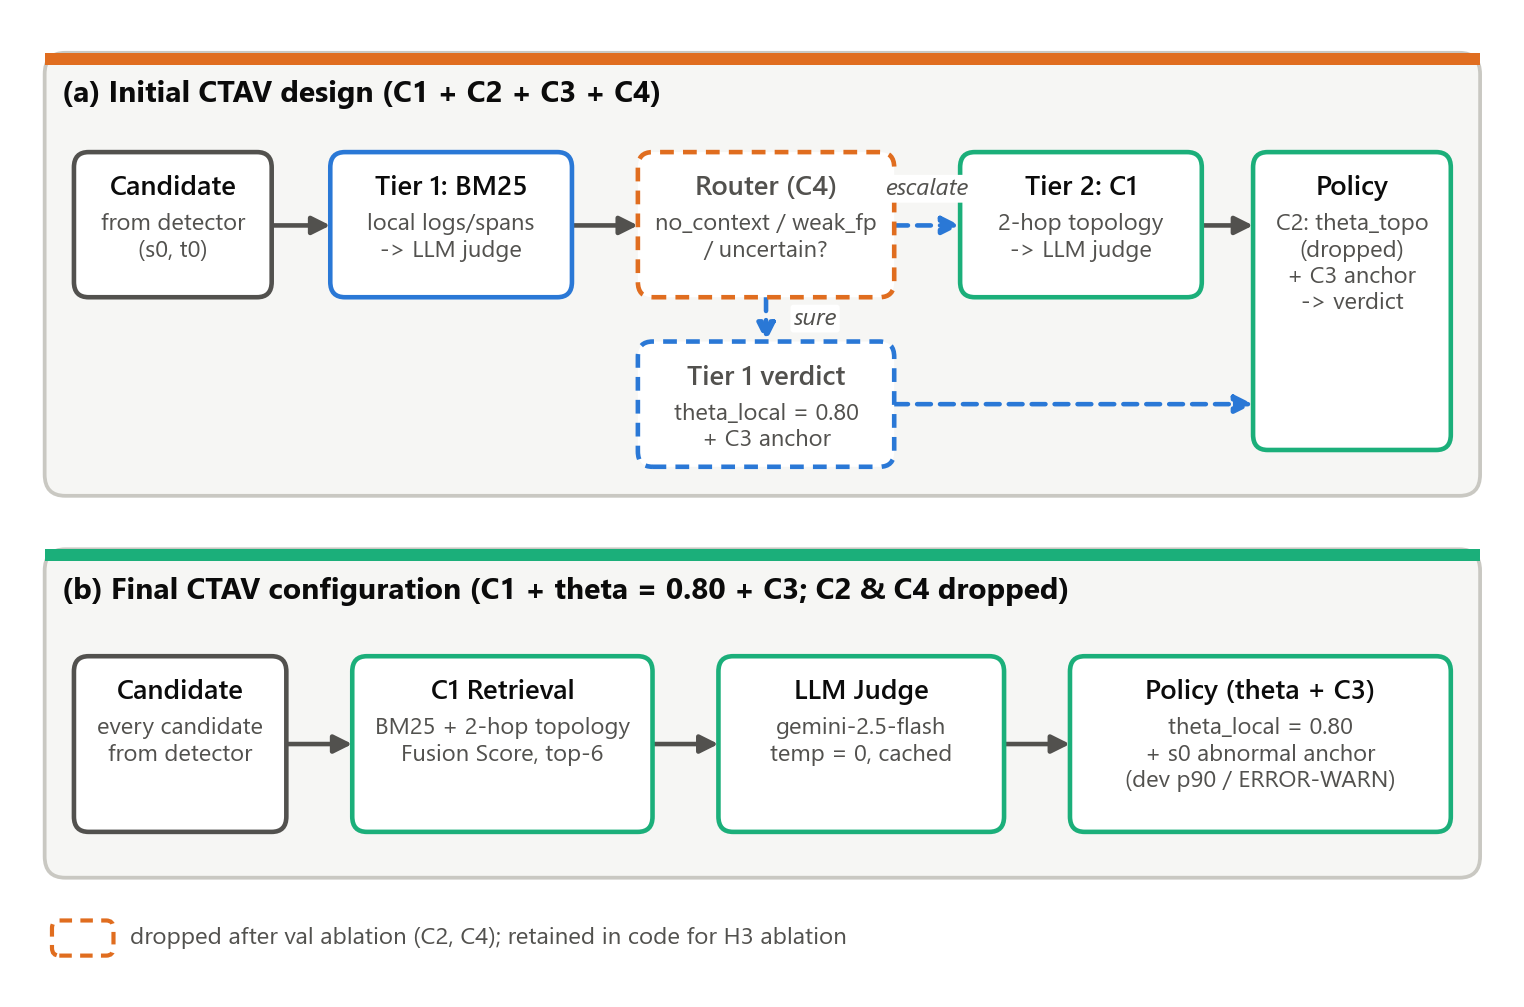
\includegraphics[width=\linewidth]{Images/C1/figures/ch4/h4.4-ctav-design-vs-final.png}
  \vspace{0.35cm}
  \caption[So sánh kiến trúc CTAV ban đầu và cấu hình chốt]{So sánh kiến trúc \CTAV{} giữa thiết kế ban đầu (a) và cấu hình chốt (b) chỉ giữ \comp{C1}, ngưỡng $\theta_{\text{local}} = 0{,}80$ và neo bằng chứng \comp{C3} (\comp{C2}, \comp{C4} đã loại). \emph{(Nguồn: tác giả vẽ, có hỗ trợ AI.)}}
  \label{fig:ch4-ctav-compare}
\end{figure}

Trên tập \splitname{val}, kiểm định loại trừ dẫn đến hai quyết định tinh gọn: loại \comp{C4} vì chạy hai tầng tốn chi phí hơn chạy thẳng \comp{C1} mà F1 không tăng, và loại \comp{C2} vì bỏ \comp{C2} không làm thay đổi đáng kể \term{FPR}{FPR} (Mục~\ref{sec:ch5-val-ctav}). Cấu hình chốt của \CTAV{} vì thế rút gọn thành: \emph{mọi ứng viên $\to$ truy xuất \comp{C1} $\to$ judge \code{gemini-2.5-flash} $\to$ ngưỡng $\theta_{\text{local}} = 0{,}80$ $\to$ neo bằng chứng \comp{C3} (ngưỡng nền \splitname{dev} $p_{90}$)}. Vai trò cố định của năm thành phần \comp{C1}--\comp{C5} được tổng kết ở Bảng~\ref{tab:ch4-c1-c5}.

\begin{table}[H]
  \centering
  \caption{Vai trò hiện tại của từng thành phần trong không gian thiết kế \CTAV{} và cổng cứu cảnh báo.}
  \label{tab:ch4-c1-c5}
  \tblfont
  \tblsetup
  \begin{tabularx}{\linewidth}{|l|Y|>{\raggedright\arraybackslash}p{2.7cm}|Y|}
    \hline
    \rowcolor{gray!15}
    \textbf{Ký hiệu} & \textbf{Chức năng} & \textbf{Vai trò hiện tại} & \textbf{Cơ sở quyết định trên \splitname{val}} \\
    \hline
    \textbf{\comp{C1}} & Truy xuất lai \term{BM25}{BM25}--topology (\term{FusionScore}{Fusion Score}) & \textbf{Đang dùng} & Tái lập lợi ích nhận diện của topology trên mọi ứng viên \\
    \hline
    \textbf{\comp{C2}} & Ngưỡng bất đối xứng theo nguồn bằng chứng ($\theta_{\text{topo}} > \theta_{\text{local}}$) & \textbf{Đã loại} & Bỏ \comp{C2} chỉ thêm 2 FP ($\Delta\text{FPR}$ CI chạm $0$) \\
    \hline
    \textbf{\comp{C3}} & Neo bằng chứng bất thường của $s_0$ (ngưỡng nền \splitname{dev} $p_{90}$) & \textbf{Đang dùng} (đóng góp chính) & Hạ mạnh FP của \comp{C1} ($606 \to 51$), tăng F1 có ý nghĩa \\
    \hline
    \textbf{\comp{C4}} & Định tuyến hai tầng thích nghi (\term{BM25}{BM25} $\to$ \comp{C1}) & \textbf{Đã loại} & Chi phí cao hơn \comp{C1} chạy thẳng ($5{,}14$ vs $3{,}28$ USD), F1 không tăng \\
    \hline
    \textbf{\comp{C5}} & Cổng cứu cảnh báo \code{Rescue Score} & \textbf{Chỉ là ablation} & Thêm 2 TP / 16 FP ($\Delta\text{F1} = +0{,}001$, CI chứa $0$) \\
    \hline
  \end{tabularx}
\end{table}

\subsubsection{\term{BM25}{BM25} cục bộ và bộ thẩm định nền}
\label{sec:ch4-bm25}

\textbf{Vấn đề giải quyết và thiết kế.} Để đối chứng đóng góp thực chất của truy xuất topology và chính sách hiệu chỉnh trên cùng tập ứng viên, mô hình judge và ngân sách $B$, hệ thống hiện thực hai chiến lược nền song song với \comp{C1} (\code{hybrid\_bm25\_graph}): (i)~\code{bm25\_hybrid} dựng truy vấn từ tên service $s_0$, ba \code{top\_features} và từ khóa lỗi chuẩn hóa (tuyệt đối không đưa nhãn lỗi vào truy vấn), tìm riêng trong log và trace span của $s_0$ trong biên $\pm 8$ phút, xếp hạng bằng \term{BM25}{BM25}~\cite{robertson2009bm25} chọn top $k = 6$ trong $4.000$ token; và (ii)~\code{no\_retrieval} trả ngữ cảnh rỗng ($E(w) = \emptyset$, tắt \code{require\_evidence}) để đo năng lực suy luận chỉ từ ảnh chụp metric ở cùng ngân sách $B$. Các biến thể ablation thời gian thuần ($\beta = 1$) hoặc đồ thị thuần ($\gamma = 1$) được cấu hình trực tiếp qua trọng số của \comp{C1} thay vì tạo lớp riêng.

\textbf{Vai trò và dẫn chiếu.} \code{bm25\_hybrid} là baseline khoa học cho \hyp{H0}, \hyp{H2} và tầng 1 của nhánh loại trừ \comp{C4}; \code{no\_retrieval} là baseline không \term{RAG}{RAG} cho \hyp{H4} (kết quả ở Mục~\ref{sec:ch5-val}, \ref{sec:ch5-test} và \ref{sec:ch5-budget}).

\subsubsection{Truy xuất nhận biết topology \comp{C1}}
\label{sec:ch4-c1}\xtarget{def:C1}

\textbf{Vấn đề giải quyết.} Khi sự cố lan truyền qua nhiều microservice, bằng chứng trực tiếp trong cửa sổ của $s_0$ có thể thưa hoặc chỉ thể hiện độ trễ tăng, trong khi lỗi gốc xuất hiện rõ ở service được gọi hoặc ở các sự kiện diễn ra sát $t_0$ nhưng ít trùng khớp từ khóa với truy vấn metric. Thành phần \textbf{\comp{C1}} (bộ truy xuất lai từ khóa--đồ thị \code{HybridBm25GraphRetriever}) mở rộng phạm vi truy xuất theo đồ thị phụ thuộc và kết hợp ba tín hiệu từ khóa, thời gian và khoảng cách đồ thị.

\textbf{Thiết kế.} Quá trình truy xuất của \comp{C1} được minh họa trên Hình~\ref{fig:ch4-c1}, tách thành hai bước độc lập là dựng bể ứng viên (\code{build\_pool}) và xếp hạng chọn lọc (\code{top\_events}) nhằm cho phép đánh giá lại nhiều bộ trọng số trên cùng một bể mà không lặp lại bước truy vấn dữ liệu. Cụ thể:
\begin{enumerate}
  \item \emph{Mở rộng vùng lân cận 2 hop:} Từ $s_0$, tìm tập service có thể tới được trong bán kính $d_G(s_i, s_0) \le 2$ trên đồ thị phụ thuộc vô hướng ($56$ service, $68$ cạnh), trong đó $d_G(s_0, s_0) = 0$. Kho dữ liệu được lọc trong khung thời gian $[t_{\text{start}} - 8\,\text{phút},\; t_{\text{end}} + 8\,\text{phút}]$ (\code{bm25\_pool = window}; chế độ \code{global} không giới hạn thời gian chỉ giữ riêng cho bước kiểm chứng hồi quy G-paper).
  \item \emph{Hợp nhất hai nguồn ứng viên:} Lấy top \code{bm25\_k = 60} sự kiện có điểm \term{BM25}{BM25} cao nhất trên kho vùng lân cận, hợp nhất và khử trùng lặp với tối đa $20$ sự kiện gần trung điểm $t_0$ nhất của mỗi service trong bán kính 2 hop. Mỗi sự kiện gắn nhãn nguồn gốc \code{origin = local} nếu $d_G = 0$, ngược lại \code{graph}.
  \item \emph{Xếp hạng \term{FusionScore}{Fusion Score} và cắt theo ngân sách:} Mỗi sự kiện $e_i = (s_i, t_i)$ trong bể ứng viên được chấm điểm hợp nhất:
  \begin{equation}
    \text{Score}(e_i, s_0, t_0) = \alpha \cdot \widehat{\text{BM25}}(e_i) + \beta \cdot \exp\!\left(-\frac{|t_i - t_0|}{\tau_F}\right) + \gamma \cdot \frac{1}{1 + d_G(s_i, s_0)},
    \label{eq:ch4-fusion}
  \end{equation}
  với $\alpha + \beta + \gamma = 1$, $\widehat{\text{BM25}}(e_i)$ là điểm \term{BM25}{BM25} chuẩn hóa min--max trên toàn bể ứng viên (bằng $1$ nếu điểm dương trên bể đồng nhất, bằng $0$ nếu điểm bằng $0$), và $\text{GraphSim} = 0$ nếu service không liên thông. Sau khi xếp hạng, hệ thống chọn top $k = 6$ sự kiện không vượt quá $4.000$ token. Tùy chọn hạn ngạch \code{k\_graph} (biến thể \comp{C1}-quota) cho phép giữ tối thiểu $\min(k_{\text{graph}}, \text{số sự kiện sẵn có})$ sự kiện \code{origin = graph}; engine vector hóa \code{WindowIndex} tăng tốc truy vấn gấp khoảng 10 lần mà cho đầu ra trùng khớp tuyệt đối với bản tham chiếu Python thuần.
\end{enumerate}

\begin{figure}[htbp]
  \centering
  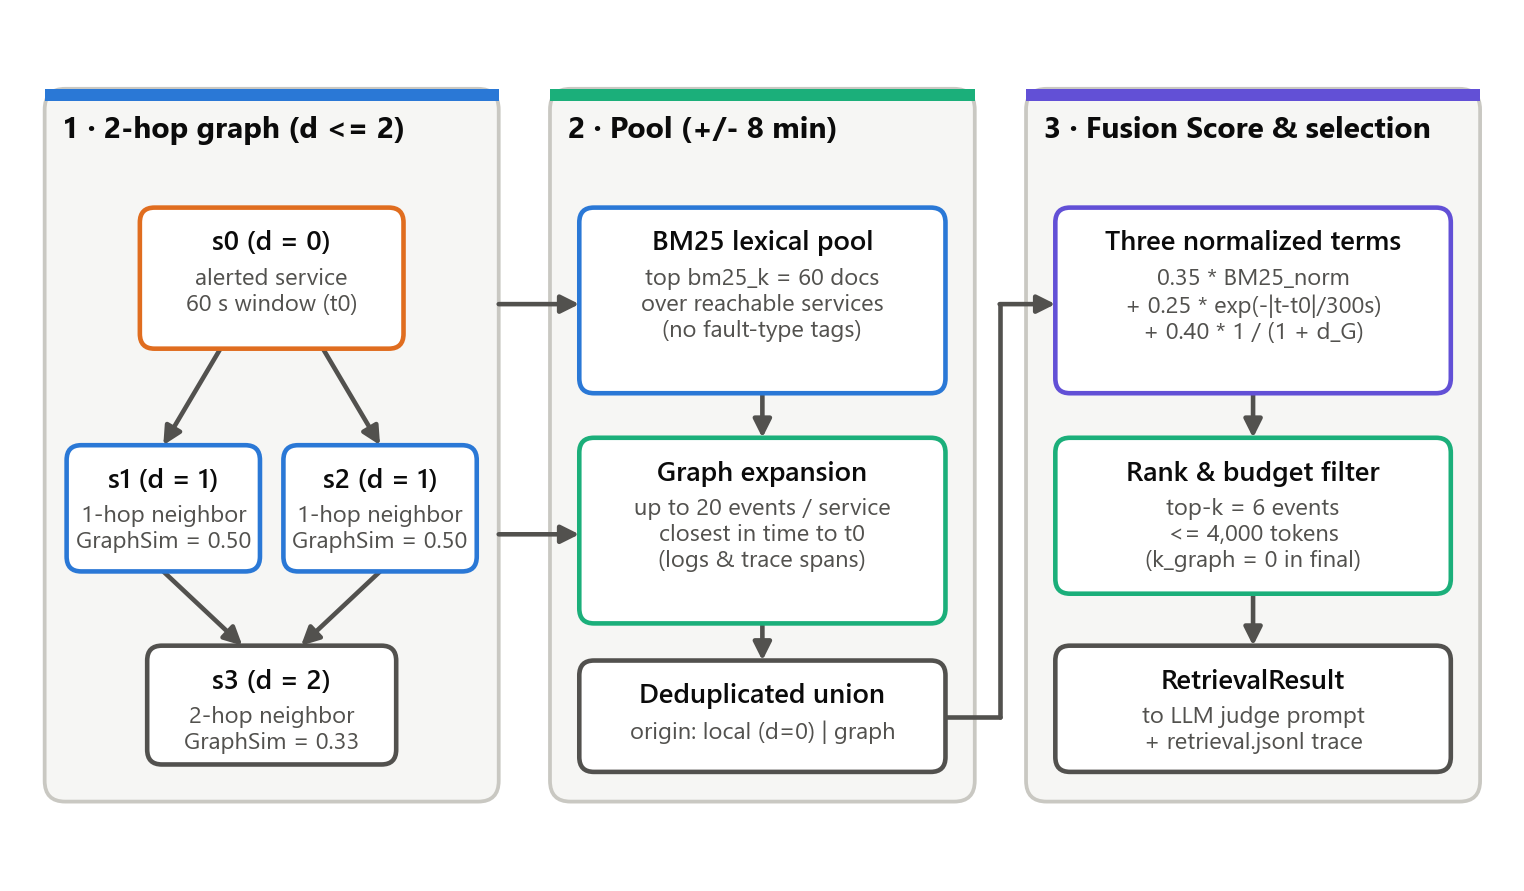
\includegraphics[width=\linewidth]{Images/C1/figures/ch4/h4.5-c1-2hop-fusion.png}
  \vspace{0.35cm}
  \caption[Cơ chế truy xuất nhận biết topology C1 và Fusion Score]{Cơ chế truy xuất nhận biết topology \comp{C1}: mở rộng 2~hop quanh $s_0$, hợp nhất bể \term{BM25}{BM25} và đồ thị ($\pm 8$~phút), xếp hạng \term{FusionScore}{Fusion Score} chọn top-6. \emph{(Nguồn: tác giả vẽ, có hỗ trợ AI.)}}
  \label{fig:ch4-c1}
\end{figure}

\textbf{Tham số, cách chọn và vai trò hiện tại.} Các tham số của \comp{C1} được tổng hợp trong Bảng~\ref{tab:ch4-pipeline-params}. Sau khi khảo sát hạn ngạch $k_{\text{graph}} \in \{0, 1, 2, 3\}$ và 32 tổ hợp trọng số trên \splitname{val} (Mục~\ref{sec:ch5-val-c1}), cấu hình chốt giữ $(\alpha, \beta, \gamma) = (0{,}35;\, 0{,}25;\, 0{,}40)$, $\tau_F = 300\,\text{s}$ và \code{k\_graph = 0} vì ép thêm bằng chứng lân cận không cải thiện độ trúng gốc hay F1. \textbf{\comp{C1} đang dùng} làm chiến lược truy xuất duy nhất của \CTAV{} (bằng chứng ở Mục~\ref{sec:ch5-val} và Mục~\ref{sec:ch5-test}).

\subsubsection{Chính sách quyết định: neo bằng chứng (\comp{C3}) và ngưỡng bất đối xứng (\comp{C2}, đã loại)}
\label{sec:ch4-policy}

\textbf{Vấn đề giải quyết.} Khi đưa ngữ cảnh từ \comp{C1} vào \emph{LLM-as-a-Judge}, mô hình ngôn ngữ có xu hướng xác nhận \code{TRUE\_ALERT} với điểm tin cậy cao ($0{,}85$--$0{,}90$) ngay cả trên các cửa sổ bình thường chỉ vì thấy các trace span nằm sát mốc $t_0$ (khảo sát \hyp{H1} trên \splitname{val}, Mục~\ref{sec:ch5-h1}). Thay vì chỉ dựa vào nhãn thô hoặc câu nhắc prompt vốn khó kiểm soát độ ổn định, tầng chính sách quyết định đặt các quy tắc định lượng tường minh sau bộ thẩm định để chặn báo động giả có hệ thống.

\textbf{Thiết kế chính sách quyết định.} Như minh họa trên Hình~\ref{fig:ch4-policy}, chính sách là một \emph{hàm thuần} nhận phán quyết thô \code{raw\_verdict}, độ tin cậy \code{confidence} và tập thông tin bằng chứng đã trích dẫn \code{cited} của từng ứng viên đã lưu cache. Mọi phán quyết thô khác \code{TRUE\_ALERT} (tức \code{FALSE\_POSITIVE}, \code{UNCERTAIN} hoặc lỗi \code{manual\_review}) đi thẳng không đổi; riêng \code{TRUE\_ALERT} phải vượt qua tuần tự ba cổng:
\begin{enumerate}
  \item \emph{Cổng kiểm tra trích dẫn (\code{require\_evidence}):} Tập \code{cited} (sau khi đã lọc bỏ mọi \code{event\_id} không tồn tại trong ngữ cảnh) phải khác rỗng; nếu rỗng thì hạ xuống \code{UNCERTAIN} với cờ \code{downgraded\_by\_evidence\_rule}.
  \item \xtarget{def:C2}\emph{Cổng ngưỡng tin cậy (và nhánh \comp{C2} đã loại):} Nếu $\text{confidence} < \theta_{\text{local}}$ ($\theta_{\text{local}} = 0{,}80$), hạ xuống \code{UNCERTAIN} (\code{downgraded\_by\_threshold}). Trong thiết kế ban đầu có bật \textbf{\comp{C2}}, các phán quyết xuất phát từ tầng topology ($tier = 2$) phải vượt ngưỡng cao hơn $\theta_{\text{topo}} = 0{,}85$; nếu $\theta_{\text{local}} \le \text{confidence} < \theta_{\text{topo}}$ thì hạ với cờ \code{downgraded\_by\_gating}.
  \item \xtarget{def:C3}\emph{Cổng neo bằng chứng bất thường (\textbf{\comp{C3}}):} Phán quyết \code{TRUE\_ALERT} chỉ được giữ khi tồn tại ít nhất một sự kiện $e \in C(w)$ thỏa vị từ bất thường của chính service phát cảnh báo $s_0$:
  \begin{equation}
    \begin{aligned}
      \text{Abnormal}(e, s_0) \iff (s_e = s_0) \land \Big[
        &\big(e \text{ là log} \land \text{level}(e) \in \{\code{ERROR}, \code{WARN}\}\big) \\
        &\lor \big(e \text{ là span} \land \text{dur}(e) > q_{90}(s_0, \text{op}_e)\big)
      \Big],
    \end{aligned}
    \label{eq:ch4-c3-anchor}
  \end{equation}
  trong đó $q_{90}(s_0, \text{op}_e)$ là phân vị thứ 90 của thời lượng \code{duration\_ms} cho cặp $(s_0, \text{op}_e)$ ước lượng từ bộ tính ngưỡng nền span. Nếu không có sự kiện nào thỏa~\eqref{eq:ch4-c3-anchor}, cảnh báo bị hạ xuống \code{UNCERTAIN} với cờ \code{downgraded\_by\_anchoring}.
\end{enumerate}

\begin{figure}[htbp]
  \centering
  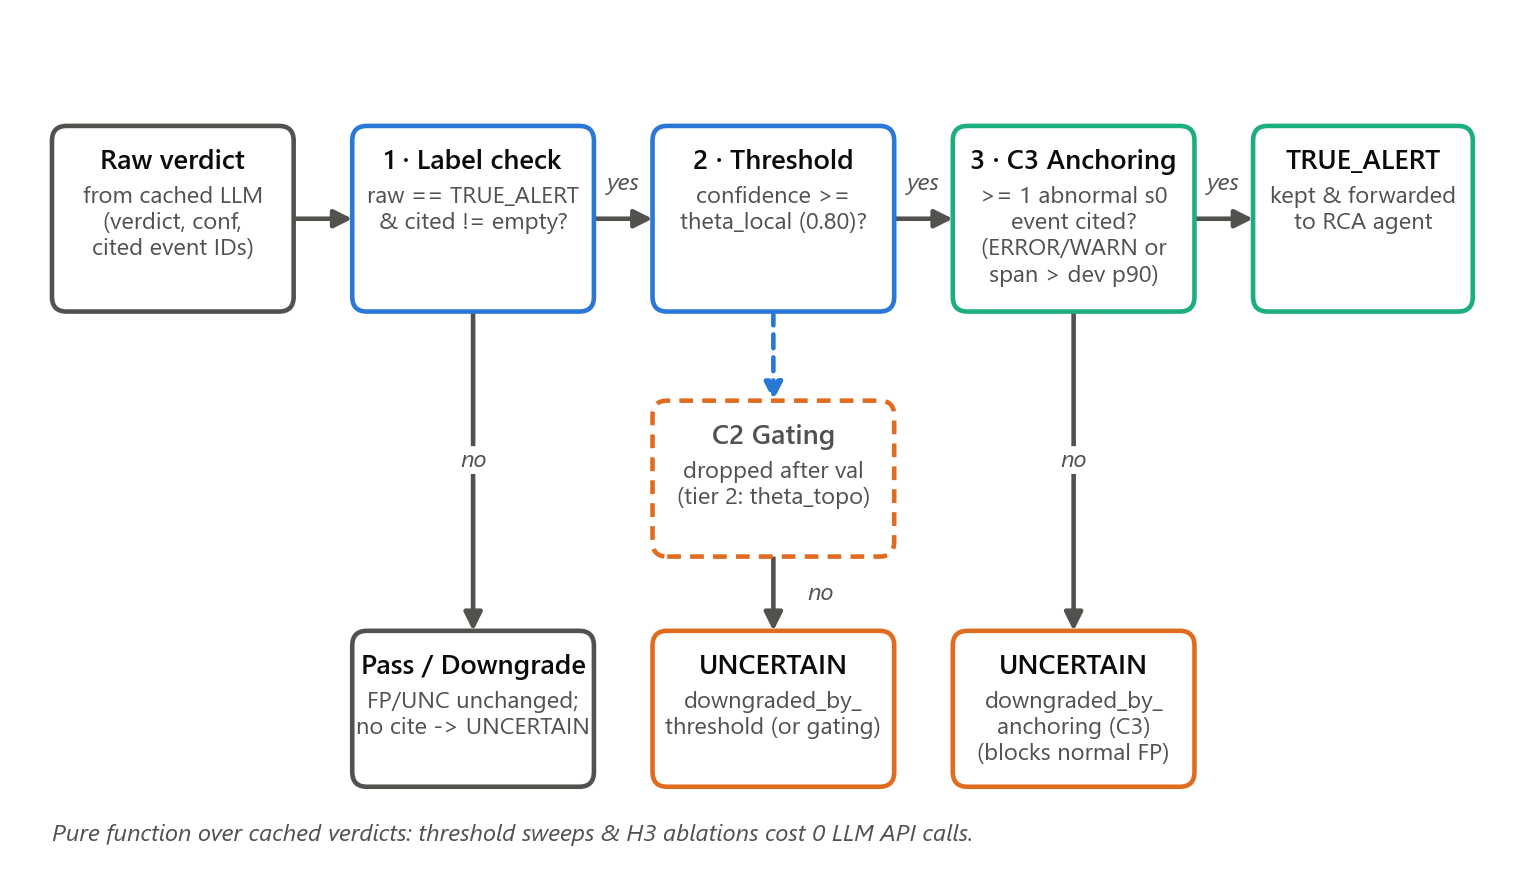
\includegraphics[width=\linewidth]{Images/C1/figures/ch4/h4.6-decision-policy.png}
  \vspace{0.35cm}
  \caption[Sơ đồ luồng chính sách quyết định CTAV]{Sơ đồ luồng chính sách quyết định \CTAV{} trên phán quyết đã lưu cache: kiểm trích dẫn, ngưỡng $\theta_{\text{local}} = 0{,}80$ (\comp{C2} nét đứt đã loại) và neo \comp{C3} tại $s_0$. \emph{(Nguồn: tác giả vẽ, có hỗ trợ AI.)}}
  \label{fig:ch4-policy}
\end{figure}

\textbf{Xây dựng ngưỡng nền và lựa chọn thiết kế.} Để ngưỡng nền $q_{90}(s_0, \text{op}_e)$ không bị nhiễm độ trễ lỗi lan truyền, bộ chọn \code{SpanSelector} chỉ giữ các trace span thuộc cửa sổ bình thường sạch trên \splitname{dev} (ngoài mọi khoảng tiêm lỗi của cùng hệ thống) với tối thiểu $\code{MIN\_SPANS} = 30$ span mỗi cặp $(s_0, \text{op}_e)$; cặp thiếu ngưỡng không thể dùng làm bằng chứng neo. Bảng~\ref{tab:ch4-policy-rules} đối chiếu các điều kiện hạ bậc cùng hai nguồn ngưỡng nền khảo sát trên \splitname{val}: theo quy tắc lựa chọn đã khóa, \CTAV{} chốt ngưỡng nền \splitname{dev} $p_{90}$ và giữ biến thể ngưỡng trượt 60 phút không cần nhãn (\code{RollingSpanBaseline}) làm đối chứng độ nhạy bắt buộc ở Chương~\ref{ch:thuc-nghiem}.

\begin{table}[H]
  \centering
  \caption{Tổng hợp các điều kiện hạ bậc của chính sách quyết định và so sánh hai nguồn ngưỡng nền cho \comp{C3}.}
  \label{tab:ch4-policy-rules}
  \tblfont
  \tblsetup
  \begin{tabularx}{\linewidth}{|>{\raggedright\arraybackslash}p{3.0cm}|Y|Y|>{\raggedright\arraybackslash}p{2.2cm}|}
    \hline
    \rowcolor{gray!15}
    \textbf{Quy tắc / Biến thể} & \textbf{Điều kiện áp dụng} & \textbf{Hành động \& ghi nhận} & \textbf{Trạng thái} \\
    \hline
    \code{require\_\allowbreak evidence} & \code{raw\_verdict == TRUE\_ALERT} nhưng không có ID trích dẫn hợp lệ & Hạ \code{UNCERTAIN} (\code{downgraded\_by\_\allowbreak evidence\_rule}) & Đang dùng \\
    \hline
    Ngưỡng $\theta_{\text{local}}$ & $\text{confidence} < 0{,}80$ & Hạ \code{UNCERTAIN} (\code{downgraded\_by\_\allowbreak threshold}) & Đang dùng \\
    \hline
    Gating \textbf{\comp{C2}} & Tầng topology ($tier = 2$) có $0{,}80 \le \text{confidence} < 0{,}85$ & Hạ \code{UNCERTAIN} (\code{downgraded\_by\_\allowbreak gating}) & \textbf{Đã loại} \\
    \hline
    Neo \textbf{\comp{C3}} (\splitname{dev} $p_{90}$) & Không có log \code{ERROR}/\code{WARN} hay span của $s_0$ vượt $q_{90}$ tính từ \splitname{dev} sạch ($\ge 30$ span) & Hạ \code{UNCERTAIN} (\code{downgraded\_by\_\allowbreak anchoring}); giữ ID neo nếu đạt & \textbf{Đang dùng} (chính) \\
    \hline
    Neo \textbf{\comp{C3}} (trượt 60 phút) & Như trên nhưng tính $q_{90}$ trên cửa sổ trượt $[t_{\text{start}} - g - 60\text{m},\; t_{\text{start}} - g)$ không cần nhãn & Phủ $\approx 93\%$ span nhưng cho F1 thấp hơn trên \splitname{val} & Ablation / độ nhạy \\
    \hline
  \end{tabularx}
\end{table}

\textbf{Vai trò hiện tại và dẫn chiếu.} \textbf{\comp{C3} đang dùng} và là đóng góp quyết định hiệu quả kìm báo động giả của \CTAV{}; \textbf{\comp{C2} đã loại} sau kiểm định \hyp{H3} trên \splitname{val}. Nhờ lưu song song phán quyết thô và phán quyết sau chính sách, mọi lần quét ngưỡng hay phân tích loại trừ đều tiêu tốn $0$ lần gọi API mới. Bằng chứng chi tiết nằm tại Mục~\ref{sec:ch5-val}, Mục~\ref{sec:ch5-test} và Mục~\ref{sec:ch5-ablation}.

\subsubsection{Định tuyến hai tầng thích nghi (\comp{C4}, đã loại)}
\label{sec:ch4-c4}\xtarget{def:C4}

\textbf{Vấn đề giải quyết.} Thành phần định tuyến hai tầng \textbf{\comp{C4}} được thiết kế ban đầu nhằm giảm chi phí gọi LLM của ngữ cảnh topology: chỉ chạy truy xuất cục bộ \term{BM25}{BM25} ở tầng 1 cho mọi ứng viên, và chỉ leo thang sang tầng 2 (\comp{C1}) đối với những ứng viên mà tầng 1 chưa đủ cơ sở kết luận.

\textbf{Thiết kế và tham số.} Hàm \code{route()} chạy tầng 1 (\term{BM25}{BM25} $\to$ judge $\to$ chính sách quyết định), tốn 1 lần gọi LLM, sau đó kiểm tra ba điều kiện leo thang theo thứ tự ưu tiên: (i) \code{no\_context} khi tầng 1 không truy xuất được sự kiện nào; (ii) \code{uncertain} khi phán quyết tầng 1 sau chính sách là \code{UNCERTAIN} (kể cả ca bị \comp{C3} hạ); và (iii) \code{weak\_fp} khi phán quyết là \code{FALSE\_POSITIVE} với độ tin cậy nhỏ hơn \code{fp\_confidence = 0,95}. Khi thỏa một trong ba điều kiện, tầng 2 chỉ được gọi nếu ngữ cảnh \comp{C1} không rỗng và ngân sách còn lại ít nhất 2 lượt gọi (gồm lượt đã dùng ở tầng 1); nếu không, phán quyết tầng 1 được giữ nguyên.

\textbf{Lý do loại, vai trò và dẫn chiếu.} Trên tập \splitname{val}, phần lớn ca thu hồi tăng thêm của \comp{C1} rơi vào nhóm tầng 1 trả \code{FALSE\_POSITIVE}, khiến bộ định tuyến phải gọi LLM hai lần trên tỷ lệ lớn ứng viên nên tốn chi phí hơn gọi thẳng \comp{C1} mà F1 không tăng (Mục~\ref{sec:ch5-val-ctav}). Do đó \textbf{\comp{C4} đã loại} khỏi cấu hình chốt của \CTAV{}, mã nguồn chỉ giữ cho nhánh loại trừ \hyp{H3} ở Mục~\ref{sec:ch5-ablation}.

\subsubsection{Bộ thẩm định LLM: prompt, đầu ra có cấu trúc và cache}
\label{sec:ch4-judge}

\textbf{Thiết kế prompt và đầu ra JSON.} Bộ đóng gói ngữ cảnh chuẩn hóa đầu vào thành chuỗi JSON nén xác định gồm \code{alert\_candidate} (định danh, cửa sổ thời gian, pod, service, điểm bất thường làm tròn 4 chữ số, \code{metric\_snapshot}, ba \code{top\_features}, danh sách đóng \code{allowed\_evidence\_ids}) và \code{related\_logs\_events} (mỗi thông điệp cắt tối đa $240$ ký tự). Cột \code{PodSuccessRate(\%)} luôn bằng $0$ do cách ghi đo trên Nezha được loại qua \code{drop\_metrics} để tránh gây báo động giả hàng loạt. Mô hình thẩm định duy nhất là \code{gemini-2.5-flash}~\cite{google2026gemini} ($\text{temperature} = 0$, \code{thinkingBudget = 0}, kiểm \code{modelVersion} mọi phản hồi), bị ràng buộc trả đúng sáu khóa JSON: \code{label} (\code{true\_alert} $\mid$ \code{false\_positive} $\mid$ \code{uncertain}), \code{severity} (\code{P1}--\code{P3} $\mid$ \code{none}), \code{confidence} $\in [0, 1]$, \code{evidence} (chỉ lấy từ \code{allowed\_evidence\_ids}), \code{reason} ($\le 25$ từ) và \code{recommended\_action} ($\le 20$ từ). Các lỗi mạng tạm thời được thử lại tối đa $5$ lần kèm giới hạn tốc độ; quá ngưỡng sẽ chuyển sang \code{manual\_review}.

\textbf{Cơ chế cache bất biến.} Mọi lời gọi đều đi qua lớp cache JSONL chỉ ghi nối tiếp với khóa băm:
\begin{equation}
  \text{key} = \text{sha256}\big(\text{provider} \mid \text{model} \mid \text{prompt} \mid \text{"max="}\langle M \rangle\text{"|t=0"}[\text{"|repeat="}r]\big),
  \label{eq:ch4-cache-key}
\end{equation}
trong đó hậu tố \code{|repeat=r} chỉ gắn khi $r > 0$ để đo độ ổn định lặp lại của mô hình (còn $r = 0$ tương thích tuyệt đối với tệp cache bài báo tiền đề~\cite{icaetm2026}). Bảng~\ref{tab:ch4-pipeline-params} tổng hợp toàn bộ tham số chốt của bộ phát hiện, truy xuất \comp{C1}, bộ thẩm định và nhánh ablation \comp{C5}; bằng chứng độ ổn định lặp lại và chi phí nằm ở Mục~\ref{sec:ch5-gpaper} và Mục~\ref{sec:ch5-repeat}.

\begin{table}[H]
  \centering
  \caption[Tổng hợp tham số cấu hình chốt của pipeline phát hiện và CTAV]{Tổng hợp tham số cấu hình chốt của bộ phát hiện, truy xuất \comp{C1}, bộ thẩm định LLM và cổng ablation \comp{C5}.}
  \label{tab:ch4-pipeline-params}
  \tblfont
  \tblsetup
  \setlength{\tabcolsep}{4pt}
  \begin{tabularx}{\linewidth}{|>{\raggedright\arraybackslash}p{2.3cm}|>{\raggedright\arraybackslash}p{3.1cm}|>{\raggedright\arraybackslash}p{3.2cm}|Y|}
    \hline
    \rowcolor{gray!15}
    \textbf{Thành phần} & \textbf{Tham số} & \textbf{Giá trị chốt} & \textbf{Vai trò / cơ sở chọn} \\
    \hline
    Isolation Forest & \code{threshold}, \code{buffer\_size} & $0{,}85$;\; $2$ ($\approx 120\,\text{s}$) & Ngưỡng chuẩn hóa $[0, 1]$ và bộ đệm cuộn; $100$ cây, \code{contamination = 0,05} trên \splitname{dev} (\code{seed = 42}) \\
    \hline
    Truy xuất \comp{C1} & $(\alpha, \beta, \gamma)$, $\tau_F$ & $(0{,}35;\, 0{,}25;\, 0{,}40)$;\; $300\,\text{s}$ & Trọng số \term{FusionScore}{Fusion Score} và suy giảm thời gian; giữ sau ablation 32 điểm trên \splitname{val} \\
    \hline
    Truy xuất \comp{C1} & \code{max\_dist}, \code{margin}, \code{top\_k}, $k_{\text{graph}}$ & $2$ hop;\; $\pm 8$m;\; $6$;\; $0$ & Bể \code{bm25\_k = 60}, $20$ sự kiện/service, giới hạn $4.000$ token; $k_{\text{graph}} = 0$ trên \splitname{val} \\
    \hline
    Judge \& Cache & Mô hình, nhiệt độ, lỗi & \code{gemini-2.5-flash}, $T = 0$ & \code{thinkingBudget = 0}, kiểm \code{modelVersion}, \code{drop\_metrics = ["PodSuccessRate(\%)"]}, retry $5$, $200$ gọi/phút, cache \code{sha256}~\eqref{eq:ch4-cache-key} \\
    \hline
    \comp{C5} (ablation) & $(\eta_1, \eta_2, \eta_3)$, $\tau$, $k_{\text{log}}$, $\sigma$, $T_{\text{active}}$ & $(0;\, 0{,}4;\, 0{,}6)$;\; $0{,}8$;\; $10$;\; $300\,\text{s}$;\; $300\,\text{s}$ & Chọn từ lưới $147$ điểm trên \splitname{val}; chỉ giữ ablation độc lập \\
    \hline
  \end{tabularx}
\end{table}

% -----------------------------------------------------------------------------
\subsection{Tác tử phân tích nguyên nhân gốc (\term{RCA}{RCA})}
\label{sec:ch4-rca}

Mục này trình bày nhánh thứ hai của nền tảng: tác tử \term{RCA}{RCA} chuyển đổi tập cảnh báo \code{TRUE\_ALERT} đã được \CTAV{} thẩm định thành các sự cố gọn gàng, xếp hạng service nghi vấn gốc và sinh báo cáo chẩn đoán có cấu trúc. Quy trình ba bước của tác tử được minh họa ở Hình~\ref{fig:ch4-rca}; điểm thiết kế quan trọng là hai bước đầu (gom nhóm và xếp hạng gốc) hoàn toàn tất định, không gọi LLM, còn bước thứ ba dùng đúng một lần gọi LLM cho mỗi sự cố để giải thích và tổng hợp khuyến nghị dưới bộ kiểm duyệt năm quy tắc.

\begin{figure}[htbp]
  \centering
  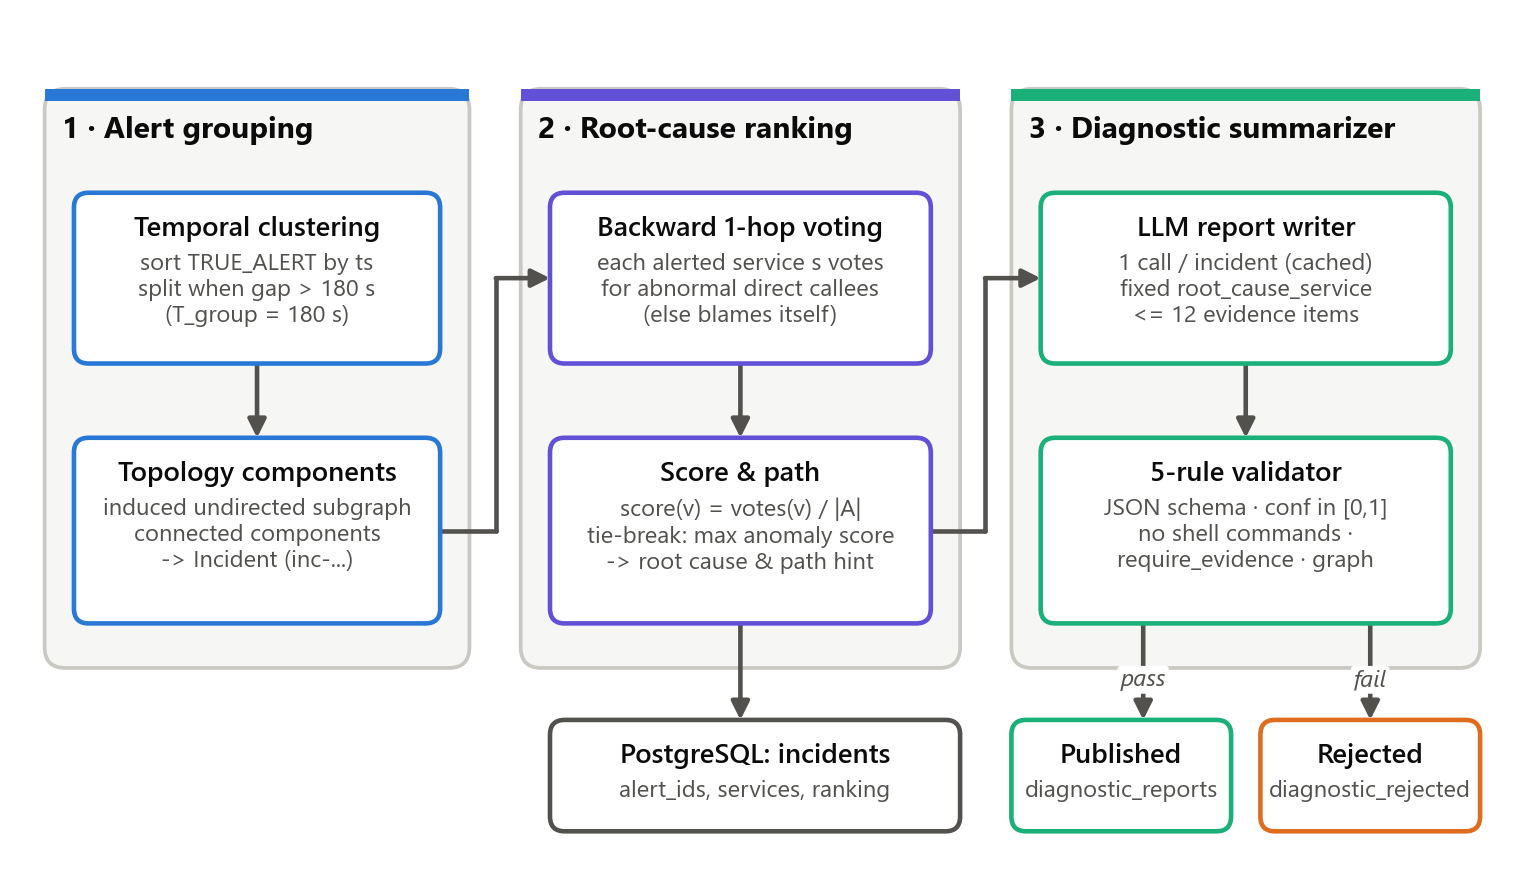
\includegraphics[width=\linewidth]{Images/C1/figures/ch4/h4.10-rca-agent.png}
  \vspace{0.35cm}
  \caption[Quy trình ba bước của tác tử RCA]{Quy trình ba bước của tác tử \term{RCA}{RCA}: gom cảnh báo ($T_{\text{group}} = 180\,\text{s}$), lan truyền ngược 1~hop và sinh báo cáo JSON qua bộ kiểm duyệt năm quy tắc. \emph{(Nguồn: tác giả vẽ, có hỗ trợ AI.)}}
  \label{fig:ch4-rca}
\end{figure}

\subsubsection{Gom cảnh báo thành sự cố}
\label{sec:ch4-grouping}

\textbf{Vấn đề giải quyết.} Một lỗi tiêm đơn lẻ thường kích hoạt nhiều cảnh báo liên tiếp trên cùng một service hoặc trên các service gọi nhau trong vài phút. Đưa từng cảnh báo rời rạc sang bước định vị gốc vừa gây trùng lặp chẩn đoán vừa làm tăng tải nhận thức cho kỹ sư vận hành.

\textbf{Thiết kế.} Thuật toán gom nhóm sự cố chạy hoàn toàn không dùng LLM theo hai bước:
\begin{enumerate}
  \item \emph{Phân cụm thời gian liên kết đơn:} Sắp xếp các cảnh báo \code{TRUE\_ALERT} tăng dần theo cặp $(t_a, \code{alert\_id})$ và tách cụm mới mỗi khi khoảng cách giữa hai cảnh báo kề nhau vượt quá ngưỡng $T_{\text{group}}$.
  \item \emph{Tách thành phần liên thông theo topology:} Trong mỗi cụm thời gian, trích đồ thị con vô hướng của đồ thị phụ thuộc $G$ cảm sinh bởi tập service có cảnh báo trong cụm (cạnh gọi theo bất kỳ chiều nào đều liên kết hai service). Mỗi thành phần liên thông tạo thành một đối tượng \code{Incident} với mã định danh tất định \code{inc-<sha256[:16]>} tính từ \code{run\_id} và danh sách \code{alert\_ids}, lưu kèm lý do gom (\code{temporal\_window\_sec} và danh sách cạnh đồ thị đã dùng). Các cảnh báo của cùng một service trong cùng cụm thời gian luôn gộp chung một sự cố.
\end{enumerate}

\textbf{Tham số, cách chọn và dẫn chiếu.} Trên tập \splitname{val}, hệ thống quét ba mức $T_{\text{group}} \in \{180, 300, 600\}\,\text{s}$ theo quy tắc lựa chọn định trước (tối thiểu số sự cố đa lỗi nhập nhằng \code{ambiguous} rồi đến \term{ARR}{ARR}). Mức $T_{\text{group}} = 180\,\text{s}$ được chốt trong cấu hình cuối của tác tử \term{RCA}{RCA} vì chỉ tạo $1$ sự cố nhập nhằng so với $2$ sự cố ở $300\,\text{s}$ và $600\,\text{s}$ (trong khi chênh lệch \term{ARR}{ARR} trên cảnh báo trong lỗi giữa $300\,\text{s}$ và $180\,\text{s}$ có CI chứa $0$). Bước gom nhóm đang dùng trong pipeline cuối và được đo bằng chỉ số \term{ARR}{ARR} ở Mục~\ref{sec:ch5-rca}.

\subsubsection{Lan truyền ngược và xếp hạng service gốc}
\label{sec:ch4-propagation}

\textbf{Vấn đề giải quyết.} Khi một sự cố gồm nhiều service có cảnh báo liên thông nhau, service chịu ảnh hưởng ở tầng trước (như cổng giao tiếp hoặc dịch vụ tổng hợp) thường có điểm bất thường cao dù lỗi gốc nằm ở dịch vụ phía sau mà nó gọi tới. Cần một thuật toán xếp hạng service gốc tận dụng chiều gọi trong đồ thị phụ thuộc để vượt qua cách xếp hạng chỉ theo điểm bất thường cực đại.

\textbf{Thiết kế.} Do phạm vi nghiên cứu ưu tiên kiểm chứng rõ ràng phương pháp tất định, đề tài hiện thực mức 1 (lan truyền ngược 1~hop \code{backward\_one\_hop}) và chủ động cắt nhánh mức 2 (dùng LLM suy luận toàn chuỗi gọi). Thuật toán khai thác quy luật lỗi lan ngược chiều gọi: khi cạnh có hướng $a \to b \in E$ tồn tại và $b$ gặp sự cố, $a$ sẽ chậm hoặc báo lỗi theo. Gọi $A$ là tập các service có cảnh báo trong sự cố và $U \supseteq A$ là tập các service có dấu hiệu bất thường trong khoảng thời gian sự cố (với cấu hình dấu hiệu \code{sign = alert} thì $U = A$; biến thể \code{sign = candidate} mở rộng thêm các service có ứng viên detector). Mỗi service $s \in A$ xác định tập đích gọi trực tiếp bất thường $\mathcal{N}^+(s) \cap U$: nếu tập này khác rỗng, $s$ chia đều $1$ phiếu bầu cho từng service trong tập đó; nếu rỗng, $s$ tự bầu $1$ phiếu cho chính mình. Điểm nghi vấn gốc của mỗi service $v$ là:
\begin{equation}
  \text{score}_{\text{RCA}}(v) = \frac{1}{|A|} \sum_{s \in A} \frac{\mathbb{I}[v \in T(s)]}{|T(s)|},
  \qquad
  T(s) =
  \begin{cases}
    \mathcal{N}^+(s) \cap U & \text{nếu } \mathcal{N}^+(s) \cap U \neq \emptyset, \\
    \{s\} & \text{ngược lại.}
  \end{cases}
  \label{eq:ch4-rca-vote}
\end{equation}
Tính phiếu theo \emph{mỗi service có cảnh báo} thay vì theo từng cảnh báo giúp thứ hạng không bị lệch nếu một service phát nhiều cảnh báo hơn các service khác. Danh sách kết quả được sắp giảm dần theo $\text{score}_{\text{RCA}}(v)$, phá hòa theo điểm bất thường cực đại của service trong khoảng sự cố rồi đến thứ tự tên service; các service trong $A$ chưa nhận phiếu vẫn được nối vào cuối danh sách để phép đo $\text{Hit}@3$ có thể đánh giá đầy đủ. Từ nút hạng 1, hàm \code{propagation\_path} dựng đường lan truyền gợi ý đi từ service gốc ra các service gọi đã bầu cho nó.

\textbf{Tham số, cách chọn và dẫn chiếu.} Trên tập \splitname{val}, mở rộng dấu hiệu bất thường sang \code{sign = candidate} chỉ tăng $+0{,}091$ $\text{Hit}@1$ với CI chạm $0$, nên cấu hình chốt giữ \code{sign = alert}. Thuật toán đang dùng trong pipeline cuối và được kiểm định đối chứng với baseline \code{rank\_by\_anomaly\_score} (xếp hạng theo điểm bất thường cao nhất trong sự cố) theo giả thuyết \hyp{H5} tại Mục~\ref{sec:ch5-rca}.

\subsubsection{Báo cáo chẩn đoán có cấu trúc JSON}
\label{sec:ch4-report}

\textbf{Vấn đề giải quyết.} Một danh sách xếp hạng tên service đơn thuần chưa đủ giúp kỹ sư trực nắm bắt loại sự cố, bằng chứng hậu thuẫn và hướng kiểm tra tiếp theo; tuy nhiên, để LLM tự do viết văn bản chẩn đoán dễ dẫn đến bịa định danh bằng chứng hoặc sinh lệnh can thiệp hệ thống nguy hiểm.

\textbf{Thiết kế và bộ kiểm duyệt.} Bộ tóm tắt chẩn đoán gọi đúng một lần API \code{gemini-2.5-flash} cho mỗi sự cố (dùng chung lớp cache JSONL với bộ thẩm định, giới hạn tối đa $1.024$ token đầu ra, truyền tối đa $12$ sự kiện bằng chứng với mỗi đoạn trích tối đa $240$ ký tự). Thiết kế tách chặt trách nhiệm: tên \code{root\_cause\_service} do hạng 1 của bước~\eqref{eq:ch4-rca-vote} ấn định và mô hình không được phép thay đổi; LLM chỉ sinh năm trường có cấu trúc theo lược đồ ở Bảng~\ref{tab:ch4-report-schema}. Để ngăn prompt thay đổi âm thầm giữa các lượt chạy, cấu hình khóa cứng mã băm dấu vân tay \code{prompt\_fingerprint = 8c1d50e6ba757ee6}. Mọi câu trả lời JSON đi qua bộ kiểm duyệt năm bước tuần tự trước khi xuất bản vào bảng \code{diagnostic\_reports}; nếu vi phạm bất kỳ quy tắc từ chối nào, bản ghi được ghi sang bảng \code{diagnostic\_rejected} kèm lý do cụ thể thay vì bỏ qua âm thầm. Tỷ lệ JSON hợp lệ được định nghĩa là số báo cáo xuất bản chia cho tổng số lần gọi LLM.

\begin{table}[H]
  \centering
  \caption{Lược đồ đầu ra \code{DiagnosticReport} và năm quy tắc kiểm duyệt tự động.}
  \label{tab:ch4-report-schema}
  \tblfont
  \tblsetup
  \begin{tabularx}{\linewidth}{|l|Y|Y|}
    \hline
    \rowcolor{gray!15}
    \textbf{Trường / Quy tắc} & \textbf{Kiểu dữ liệu \& ràng buộc} & \textbf{Xử lý khi vi phạm} \\
    \hline
    \code{fault\_type} & Một trong \code{network\_delay}, \code{cpu\_contention}, \code{exception}, \code{unknown} & Từ chối (\code{invalid\_json}) nếu ngoài danh mục \\
    \hline
    \code{confidence} & Số thực trong đoạn $[0, 1]$ & Từ chối (\code{confidence\_out\_of\_range}) \\
    \hline
    \code{evidence} & Danh sách 1--4 mã \code{event\_id} thuộc \code{allowed\_evidence\_ids} & Loại mã bịa đặt; nếu không còn mã hợp lệ $\to$ từ chối (\code{no\_evidence}) \\
    \hline
    \code{propagation\_path} & Chuỗi tên service từ gốc ra ngoài & Giữ đúng lược đồ chuỗi tên service trong prompt \\
    \hline
    \code{suggested\_actions} & 1--3 câu tiếng Anh ($\le 25$ từ) kèm mức ưu tiên \code{high}/\code{medium}/\code{low} & Chặn mọi từ lệnh (\code{kubectl}, \code{sudo}, \code{docker}, \code{rm}...) và cú pháp shell (\code{\&\&}, \code{||}, \code{\$(}) $\to$ từ chối (\code{executable\_action}) \\
    \hline
    Kiểm đồ thị dịch vụ & Kiểm \code{root\_cause\_service} $\in V$ & Vẫn xuất bản nhưng gắn cờ cảnh báo \code{suspicious = True} \\
    \hline
  \end{tabularx}
\end{table}

\textbf{Vai trò hiện tại và dẫn chiếu.} Bộ tóm tắt và kiểm duyệt JSON đang dùng trong toàn bộ luồng \term{RCA}{RCA} và dashboard sự cố; tỷ lệ JSON hợp lệ được báo cáo ở Mục~\ref{sec:ch5-rca} và chất lượng nội dung báo cáo được phân tích ở Chương~\ref{ch:thao-luan}.

% -----------------------------------------------------------------------------
\subsection{Hiện thực hóa hệ thống và harness thực nghiệm}
\label{sec:ch4-impl}

Các công nghệ thành phần đã được giới thiệu lý do lựa chọn ở Mục~\ref{sec:ch2-cong-nghe}; mục này mô tả cách tổ chức mã nguồn, lắp ráp hạ tầng lưu trữ--giao diện và vận hành harness thực nghiệm để mọi kết quả ở Chương~\ref{ch:thuc-nghiem} và kịch bản trình diễn ở Chương~\ref{ch:platform} đều tái lập được.

\textbf{Tổ chức kiến trúc mô-đun và lưu trữ hai nhánh.} Hệ thống được phân tách thành ba tầng rõ ràng: (i)~tầng thư viện lõi chứa mô hình dữ liệu Pydantic, bốn giao diện lõi, đồ thị \code{ServiceGraph} và lớp lưu trữ; (ii)~tầng dịch vụ chứa chuỗi xử lý luồng (phát lại dữ liệu, phát hiện bất thường, truy xuất ngữ cảnh, thẩm định LLM, tác tử \term{RCA}{RCA}), máy chủ API FastAPI chỉ đọc gồm tám endpoint và ứng dụng web React + TypeScript năm màn hình; (iii)~tầng thực nghiệm chứa cấu hình YAML, harness chạy thử nghiệm và kho kết quả bất biến. Toàn bộ hạ tầng đóng gói trong bốn container Docker Compose (\code{clickhouse}, \code{postgres}, \code{api}, \code{web}) hỗ trợ chạy ngoại tuyến từ cache (\code{DEMO\_OFFLINE=1}). Pipeline hợp nhất ghi đồng thời sang ClickHouse (bảng sự kiện \code{fact\_alert\_evaluation}, \code{fact\_retrieval\_trace}) và PostgreSQL (bảng quan hệ \code{run\_registry}, \code{incidents}, \code{diagnostic\_reports}, \code{diagnostic\_rejected}), kèm kiểm tra tự động \code{check\_parity} khớp $100\%$ với kết quả harness.

\textbf{Harness điều khiển bằng cấu hình và kỷ luật tái lập.} Toàn bộ thực nghiệm đều được điều khiển tập trung từ tệp cấu hình YAML thay vì gán cứng tham số trong mã nguồn; mỗi lượt chạy gắn \code{run\_id} bất biến và xuất đầy đủ tệp chứng cứ tái lập (chi tiết các lệnh vận hành và bộ kiểm thử tự động liệt kê tại Bảng~\ref{tab:ch4-harness}, Phụ lục~\ref{app:config}). Trước khi mở cổng kiểm định một lần duy nhất trên \splitname{test} (G-test), pipeline bắt buộc vượt qua hai cổng kỹ thuật G-port (Mục~\ref{sec:ch5-gport}) và G-paper (Mục~\ref{sec:ch5-gpaper}).

% -----------------------------------------------------------------------------
\subsection{Kết chương}
\label{sec:ch4-ket-chuong}

Chương này đã trình bày hoàn chỉnh thiết kế và hiện thực hóa của nền tảng AIOps gồm bốn khâu từ phát hiện bất thường đến trực quan hóa sự cố. Trong nhánh thẩm định cảnh báo, cấu hình \CTAV{} chốt sau quá trình kiểm chứng tách biệt trên tập \splitname{val} gồm bộ phát hiện Isolation Forest (ngưỡng $0{,}85$), truy xuất lai \term{BM25}{BM25}--topology \textbf{\comp{C1}} ($\alpha = 0{,}35$, $\beta = 0{,}25$, $\gamma = 0{,}40$, $\tau_F = 300\,\text{s}$, bán kính 2 hop), bộ thẩm định \code{gemini-2.5-flash} qua cache bất biến, ngưỡng tin cậy $\theta_{\text{local}} = 0{,}80$ và quy tắc neo bằng chứng bất thường \textbf{\comp{C3}} dựa trên ngưỡng nền \splitname{dev} $p_{90}$. Ba cơ chế khác trong không gian thiết kế đã được ghi nhận rõ vai trò thực tế: ngưỡng bất đối xứng \textbf{\comp{C2}} và định tuyến hai tầng \textbf{\comp{C4}} đã bị loại sau kiểm định loại trừ trên \splitname{val}, còn cổng cứu cảnh báo \textbf{\comp{C5}} (\code{Rescue Score}) chỉ giữ làm phân tích loại trừ độc lập. Ở nhánh phân tích nguyên nhân gốc, tác tử \term{RCA}{RCA} ghép nối ba bước gồm gom cảnh báo theo thời gian ($T_{\text{group}} = 180\,\text{s}$) và thành phần liên thông đồ thị, bỏ phiếu lan truyền ngược 1 bước theo chiều gọi (\code{sign = alert}), và sinh báo cáo JSON có kiểm duyệt năm quy tắc qua cùng lớp cache. Toàn bộ phương pháp đã được đóng gói vào harness điều khiển bằng cấu hình YAML cùng bộ lưu trữ ClickHouse/PostgreSQL để sẵn sàng cho bước kiểm định định lượng các giả thuyết \hyp{H0}--\hyp{H5} trong Chương~\ref{ch:thuc-nghiem}.
